\documentclass[12pt]{article}
\usepackage[hscale=0.8,vscale=0.8]{geometry}
\usepackage{amsmath}
\usepackage{amssymb}
\usepackage{listings}
\usepackage{tikz}
\usepackage{color}

\definecolor{dkgreen}{rgb}{0,0.6,0}
\definecolor{gray}{rgb}{0.5,0.5,0.5}
\definecolor{mauve}{rgb}{0.58,0,0.82}

\lstset{frame=tb,
  language=Python,
  aboveskip=3mm,
  belowskip=3mm,
  showstringspaces=false,
  columns=flexible,
  basicstyle={\small\ttfamily},
  numbers=none,
  numberstyle=\tiny\color{gray},
  keywordstyle=\color{blue},
  commentstyle=\color{dkgreen},
  stringstyle=\color{mauve},
  breaklines=true,
  breakatwhitespace=true,
  tabsize=3
}

\setlength{\parskip}{1em}

\pagenumbering{gobble}

\begin{document}
	Let $k=3$. An element of $P$ would be of the form $$f(x,y)=a_1 x^3+a_2 x^2 y+a_3 x y^2+a_4 y^3+a_5 x^2+a_6 xy+a_7 y^2+a_8 x+a_9 y+a_{10}$$
	Consider the hermite element.
	
	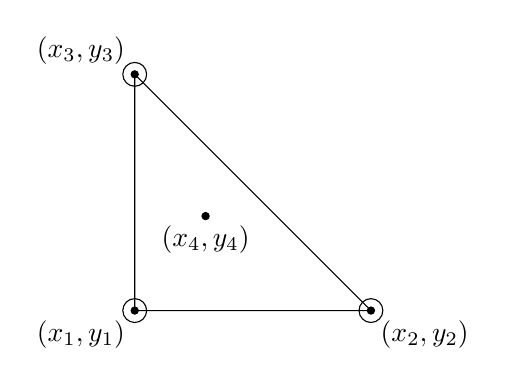
\begin{tikzpicture}
		\draw node[anchor=north east]{$(x_1,y_1)$} (0,0) --  (3,0) node[anchor=north west]{$(x_2,y_2)$} -- (0,3) node[anchor=south east]{$(x_3,y_3)$} -- (0,0);
		\draw[black,fill=black] (0,0) circle (.3ex);
		\draw[black] (0,0) circle (1ex);
		\draw[black,fill=black] (3,0) circle (.3ex);
		\draw[black] (3,0) circle (1ex);
		\draw[black,fill=black] (0,3) circle (.3ex);
		\draw[black] (0,3) circle (1ex);
		\draw[black,fill=black] (.9,1.2) circle (.3ex) node[anchor=north]{$(x_4,y_4)$};
	\end{tikzpicture}
	
	Let $\{N_1,N_2,...,N_{10}\}$ be a subset of the dual of $P$ such that for $f \in P$,
	
	$N_1(f)=f(x_1,y_1); \;\;\; N_2(f)=f(x_2,y_2); \;\;\; N_3(f)=f(x_3,y_3); \;\;\; N_4(f)=f(x_4,y_4); $
	
	$N_5(f)=\frac{\partial f}{\partial x}(x_1,y_1); \;\;\; N_6(f)=\frac{\partial f}{\partial x}(x_2,y_2); \;\;\; N_7(f)=\frac{\partial f}{\partial x}(x_3,y_3);$
	
	$N_8(f)=\frac{\partial f}{\partial y}(x_1,y_1); \;\;\; N_9(f)=\frac{\partial f}{\partial y}(x_2,y_2); \;\;\; N_{10}(f)=\frac{\partial f}{\partial y}(x_3,y_3);$
	
	The nodal basis for $P$ is $\{\phi_1,\phi_2,...,\phi_{10}\}$ such that $N_i(\phi_j)=\delta_{ij} \;\;\; \forall i,j \in \{1,2,...,10\}$
	
	To find a $\phi_4$, assume $$\phi_4(x,y)=a_1 x^3+a_2 x^2 y+a_3 x y^2+a_4 y^3+a_5 x^2+a_6 xy+a_7 y^2+a_8 x+a_9 y+a_{10}$$
	
	Then solve the following:
	$$
	\begin{bmatrix}
	x_1^3 & x_1^2 y_1& x_1 y_1^2& y_1^3& x_1^2& x_1y_1& y_1^2& x_1& y_1& 1\\[0.15cm]
	x_2^3 & x_2^2 y_2& x_2 y_2^2& y_2^3& x_2^2& x_2y_2& y_2^2& x_2& y_2& 1\\[0.15cm]
	x_3^3 & x_3^2 y_3& x_3 y_3^2& y_3^3& x_3^2& x_3y_3& y_3^2& x_3& y_3& 1\\[0.15cm]
	x_4^3 & x_4^2 y_4& x_4 y_4^2& y_4^3& x_4^2& x_4y_4& y_4^2& x_4& y_4& 1\\[0.15cm]
	
	3x_1^2 & 2x_1y_1 & y_1^2& 0& 2x_1& y_1& 0& 1& 0& 0\\[0.15cm]
	3x_2^2 & 2x_2y_2 & y_2^2& 0& 2x_2& y_2& 0& 1& 0& 0\\[0.15cm]
	3x_3^2 & 2x_3y_3 & y_3^2& 0& 2x_3& y_3& 0& 1& 0& 0\\[0.15cm]
	
	0 & x_1^2 & 2x_1 y_1& 3y_1^2& 0& x_1& 2y_1& 0& 1& 0\\[0.15cm]
	0 & x_2^2 & 2x_2 y_2& 3y_2^2& 0& x_2& 2y_2& 0& 1& 0\\[0.15cm]
	0 & x_3^2 & 2x_3 y_3& 3y_3^2& 0& x_3& 2y_3& 0& 1& 0\\[0.15cm]
	\end{bmatrix}
	\begin{bmatrix} a_1\\[0.15cm]a_2\\[0.15cm]a_3\\[0.15cm]a_4\\[0.15cm]a_5\\[0.15cm]a_6\\[0.15cm]a_7\\[0.15cm]a_8\\[0.15cm]a_9\\[0.15cm]a_{10} \end{bmatrix}
	=\begin{bmatrix} 0\\[0.15cm]0\\[0.15cm]0\\[0.15cm]1\\[0.15cm]0\\[0.15cm]0\\[0.15cm]0\\[0.15cm]0\\[0.15cm]0\\[0.15cm]0 \end{bmatrix}
	$$
	We need to calculate the inverse of the square matrix $M$ only once. After that, we can get the coefficients of the polynomial $\phi_l$ by taking the $l^{th}$ column of the inverse matrix.
	$$
	[a_i]_{10\times 1}=M^{-1} [\delta_{il}]_{10\times 1}
	$$
	Program for finding $M$:
	\begin{lstlisting}
		import os
	\end{lstlisting}
\end{document}
